\documentclass[10pt,a4paper,twoside, french]{article}
\addtolength{\textheight}{90pt} \addtolength{\topmargin}{-60pt}
\textwidth 164mm \oddsidemargin -2mm \evensidemargin -2mm
\usepackage[utf8]{inputenc}
\usepackage[T1]{fontenc}
\usepackage[english]{babel}
\usepackage{enumerate}
\usepackage{graphicx} 
\usepackage[left=2.5cm,right=2.5cm,top=3.5cm,bottom=3.5cm]{geometry}
%\usepackage{xcolor,rotating,epic,eepic}
\usepackage[font=small,labelfont=bf]{caption}  %% titre dans les minipage
\usepackage{subcaption} %% les sous figure pour les sous legendes
\usepackage{mathtools}   %%   package mathematique
\usepackage{amssymb}  %% symbole mathematique
\usepackage{fancyhdr}  %% pour pied de page et entete et layout
\usepackage{fourier}  %%  police
\usepackage{titlesec}  %% modifier les section
\usepackage{pgfplots} %% provides tools to generate plots and labeled axes easily
\usepackage{color}

\usepackage{tikz}  %%pour les figures
\usetikzlibrary{positioning}
\usepgfplotslibrary{external}
\tikzsetexternalprefix{External-TikZ/}
\tikzexternalize
\tikzset{math3d/.style=
    {y= {(0.353cm,0.353cm)}, z={(0cm,1cm)},x={(1cm,0cm)}}}
\usepackage[colorlinks = true,
            linkcolor = blue,
            urlcolor  = blue,
            citecolor = black,
            anchorcolor = blue]{hyperref} %% permet de renvoyer à la section en cliquant sur la table des matieres
            
            
            
%ecriture des algo
\usepackage{listings}
\lstset{
	language= Matlab,  %choix du language
    frame=tb, % tb=draw a frame at the top and bottom  - single=around
    tabsize=4, % tab space width
    breaklines=true,
    showstringspaces=false, % don't mark spaces in strings
    backgroundcolor=\color{gray!10},
    numbers=none, % display line numbers on the left
%    numbersep=10pt,                   % how far the line-numbers are from the code
%    numberstyle=\normal\color{black}, % the style that is used for the line-numbers
    commentstyle=\color{red}, % comment color
    keywordstyle=\color{blue}, % keyword color
    stringstyle=\color{green}, % string color
    xleftmargin=17pt,
    framexleftmargin=17pt,
    framexrightmargin=0pt,
    framexbottommargin=5pt,
    framextopmargin=5pt,
    escapeinside={(*}{*)}
}
\DeclareCaptionFormat{listing}{\hrulefill\par\vskip1pt#1#2#3}
\captionsetup[lstlisting]{format=listing,singlelinecheck=false, margin=0pt, font={sf},labelfont=bf}
%font={sf}  labelsep=space   %option captionsetup, ,\rule{\dimexpr\textwidth\relax}{0.4pt}

\renewcommand\lstlistingname{Algorithm}  % CHANGER NOM LISTING EN ALGORITHM
%%%%%%%%  Style subsection  %%%%%%%%%%
\usepackage{titlesec}  %% modifier les section
\titleformat*{\section}{\bf}
\titleformat*{\subsection}{\rm}

\numberwithin{equation}{section}
\numberwithin{figure}{section}
\numberwithin{table}{section}

%%%%%%%%%%%  COMMANDE  %%%%%%%%%%%%%%%%%%%%%%%
\newcommand{\vect}[1]{\mathbf{#1}}
\newcommand{\eq}{\Longleftrightarrow}
\newcommand{\chap}[1]{\widehat{#1}}
\newcommand{\R}{\mathbb{R}}
\newcommand{\N}{\mathbb{N}}
\newcommand{\Po}{\mathbb{P}}
\newcommand{\EspAp}[1]{\text{\textbf{#1}}_h}
\newcommand{\enstq}[2]{\left\{#1\mathrel{}\middle|\mathrel{}#2\right\}}
\newcommand{\nm}{|\!|\!|}
\newcommand{\norme}[1]{\left\Vert #1\right\Vert}
\renewcommand{\div}[1]{\text{div } \vect{#1}}
\newcommand{\rot}[1]{\text{\textbf{rot} } \vect{#1}}
\newcommand{\grad}[1]{\text{\textbf{grad} } \vect{#1}}
\newcommand{\diff}{\mathop{ }\mathopen{ }\mathrm{d}}
\newcommand{\restreinta}[1]{\mathclose{}|\mathopen{}_{#1}}
\newcommand{\prodscal}[2]{\left( #1\ ,\ #2\right)}


\begin{document}


	\vspace{1cm}    
    \begin{center}
       		\rule{10cm}{1pt} \\[0.6cm]         %% ligne horizontale   \rule[raise-height]{width}{thickness}  
        	{\huge Homework Assignment 1 \\[0.2cm]
         \Large  Numerical analysis for PDE's\\[0.2cm] 
          \large Davoud Saffar Shamshirgar - Thomas Frachon}  \\[0.6cm]
    		\rule{10cm}{1pt} \\[0.5cm]  
	\end{center}    
	
\setcounter{section}{1}
\begin{enumerate}
\item \begin{enumerate}[a.]
\item Here we consider the boundary value problem of the Eikonal equation in 1D.
\begin{align*}
\left\{
	\begin{array}{ll}
		|u_x|= r >0, & 0<x<1 \\
		u(0) = 0, \\
		u(1) = 0.
	\end{array}
\right.
\end{align*}
We solve the discretized system by a time marching method and with zero initial condition. The result of this is shown in figure \ref{fig:task1}.
\begin{figure}[h]
\centering
\includegraphics[scale=1.5]{fig/Task1}
\caption{The time marching method is  used to solve the Eikonal equation. $\Delta x=0.01$ and $\Delta t=0.01$ and $CFL=\frac{\Delta x}{\Delta t}=1$.}
\label{fig:task1}
\end{figure}

To guarantee the convergence, we need to compute the CFL condition. The discrete system for the time dependent Eikonal equation $u_t=|u_x|$, can be written as
\begin{align*}
u_j^{n+1}=&u_j^n-\frac{\Delta t}{\Delta x} \max(u_{j+1}^n-u_j^n,u_{j-1}^n-u_j^n,0)+{\cal O}(\Delta x\Delta t+\Delta t^2) \\
=&(1-\alpha)u_j^n+\alpha\max(u_{j+1}^n,u_{j-1}^n,0)+{\cal O}(\Delta x\Delta t+\Delta t^2),
\end{align*}
where $\alpha=\frac{\Delta t}{\Delta x}$. For the sake of convergence, we need to have that $\alpha\leq 1$. Hence $\Delta t\leq  \Delta x$ guarantees the convergence. We used the maximum time step to compute the solutions in figure \ref{fig:task1}.

\item Here we solve the Eikonal equation using Jacobi iterations. We observe that the total number of iterations are 21. The result showing the solutions in different iterations is shown in figure \ref{fig:task2}.
\begin{figure}[h]
\centering
\includegraphics[scale=1.5]{fig/Task2}
\caption{The solution is computed using Jacobi iterations. $\Delta x=0.01$ and $\Delta t=0.01$ and $CFL=\frac{\Delta x}{\Delta t}=1$.}
\label{fig:task2}
\end{figure}

\item Now we use Gauss-Seidel iterations to compute the solution. The scheme converges in only 2 iterations. This a considerable difference compared to the Jacobi iteration.

Note that if the initial conditions are chosen to be 2 or -2 instead of 0, the solutions for each method and number of iterations remain the same. 

\item We fix the grid and define the error as 
\begin{align*}
e_j^ n:=u(x_j)-u_j^n, u(x):= \min(|x|,|x-1|). 
\end{align*}
\begin{figure}[h]
\centering
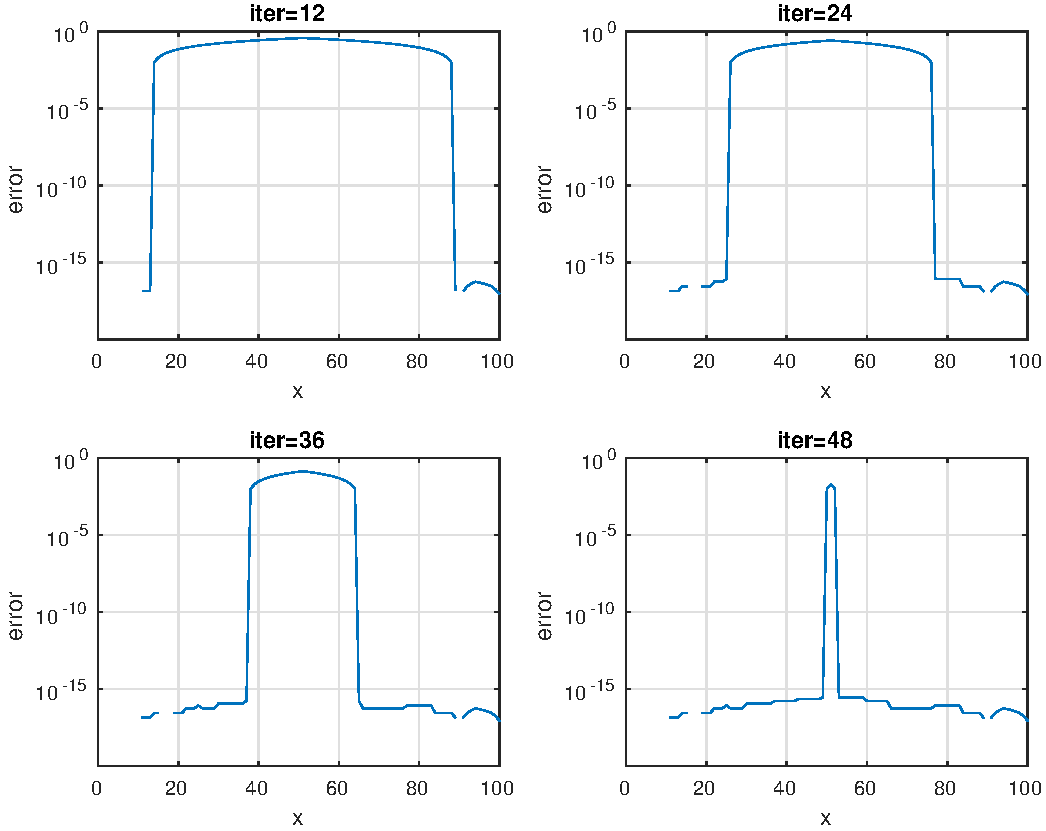
\includegraphics[scale=.7]{fig/task1_error}
\caption{Point-wise error for the time-marching method.}
\label{fig:task1_err}
\end{figure}

\begin{figure}[h]
\centering
\includegraphics[scale=.7]{fig/task2_error}
\caption{Point-wise error for the the Jacobi iterations.}
\label{fig:task2_err}
\end{figure}
\begin{figure}[h]
\centering
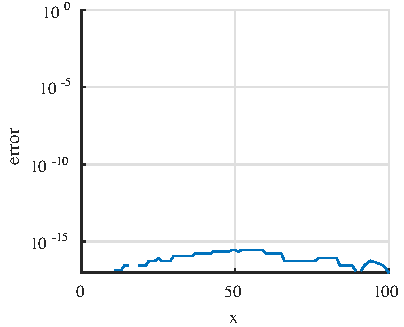
\includegraphics[scale=1]{fig/task3_error}
\caption{Point-wise error for the Gauss-Seidel iterations.}
\label{fig:task3_err}
\end{figure}

we note here that the error is very similar for the case of the Jacobi iterations and the time marching scheme. But it is certainly different for the Gauss-Seidel iterations.
\item The number of iterations is 21 for the Jacobi iteration and is 1 for the Gauss-Seidel iteration.

\item The rate of convergence is 1 for the Jacobi iteration and is 2 for the Gauss-Seidel iterations. The order of accuracy cannot be determined since the we get the exact solution for any $h$.
\end{enumerate}

\setcounter{section}{2}
\item We consider the scheme
\begin{align*}
U^{n+1} & = Q(t_n)U^n+\Delta t F^n \\
U^0 & = g
\end{align*}
We want to prove by induction that the discrete Duhamel's Principle holds.\\
The case $n=0$ is clear. Let now assume that the statement is true for a certain $n >0$. Then
\begin{align*}
U^{n+1} & = Q(t_n) \left[ S_h(t_n,0) + \Delta t \sum_{\nu =0}^{n-1} S_h(t_n,t_{\nu+1})F^\nu   \right] \\
 & = S_h(t_{n+1},0) + \Delta t \sum_{\nu=0}^{n-1} S_h(t_{n+1},t_{\nu +1})F^\nu + \Delta t F^n \\
 & = S_h(t_{n+1},0) + \Delta t \sum_{\nu=0}^n S_h(t_{n+1},t_{\nu+1})F^\nu
\end{align*}
Finally we can conclude that the statement is true for all $n \geq 0$.

\setcounter{section}{3}
\item  \begin{enumerate}[a.]
\item We consider the scalar model probelm for IVPs
\begin{align*}
\dfrac{dy}{dt} &= \lambda y,\quad \lambda>0,\\
y(0) &= 1.
\end{align*}
We try Explicit and Implicit Euler methods for the model problem. In figure \ref{fig:eeie_sol} and \ref{fig:eeie_err} we plot the solution and relative error for both methods respectively. The relative error is computed via 
\begin{align*}
e_n := \dfrac{y(t_n)-y_n}{|y(t_n)|}.
\end{align*}
\begin{figure}[h]
\centering
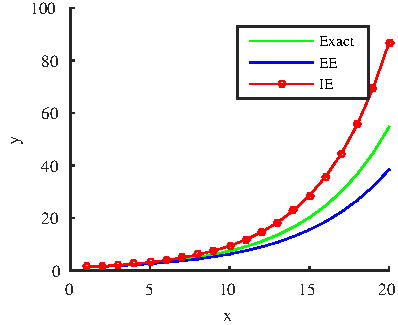
\includegraphics[scale=1]{fig/eeie_sol}
\caption{The exact, and approximate solutions using Explicit and Implicit Euler methods for $h\lambda=0.1$ (A stable solution).}
\label{fig:eeie_sol}
\end{figure}
\begin{figure}[h]
\centering
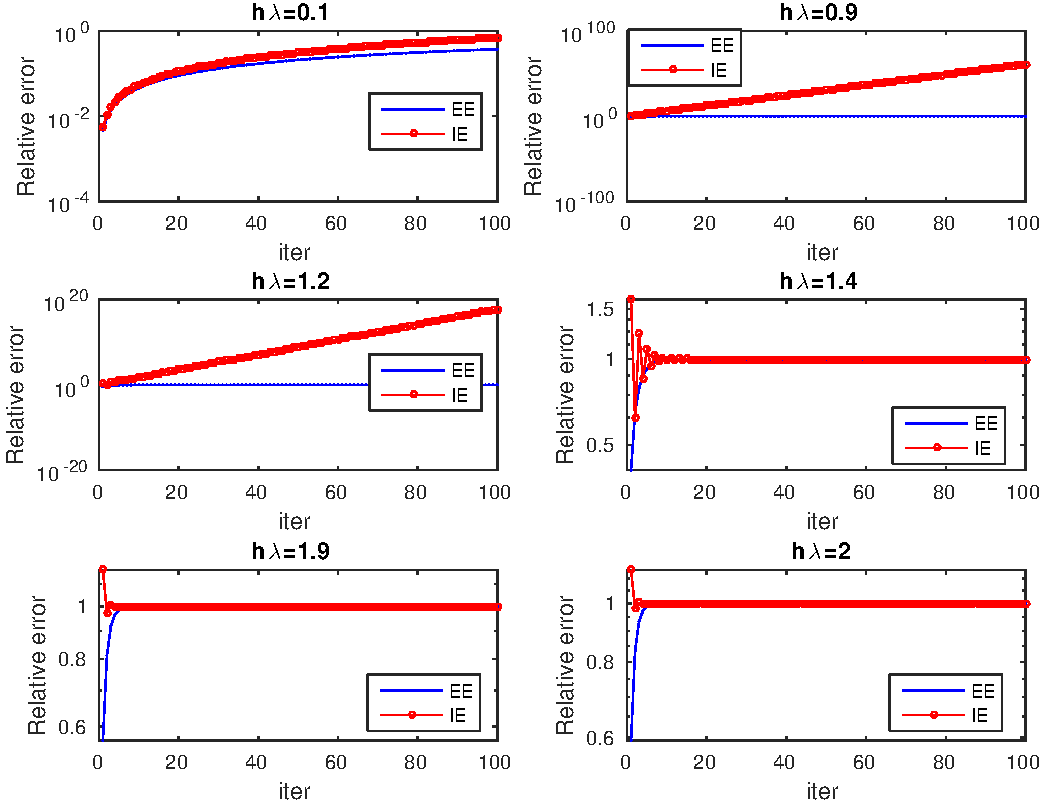
\includegraphics[scale=.9]{fig/eeie_errors}
\caption{The relative error in computing the solution of the IVP model problem using Explicit and Implicit Euler methods for different values of $h\lambda$.}
\label{fig:eeie_err}
\end{figure}

The iterations of the explicit and implicit Euler methods can be written as
\begin{align}
y_{n} &= (1+h\lambda)y_{n-1}=(1+h\lambda)^ny_0=(1+h\lambda)^n. \\
y_{n} &= (1-h\lambda)^{-1}y_{n-1}=(1-h\lambda)^{-n}y_0=(1-h\lambda)^{-n}.
\end{align}
On the other hand, the exact solution, considering the initial condition can be written as $y=e^{\lambda t}$ and $y(t_n)=e^{\lambda nh}$. Now we can compute the error for both methods.
\begin{align}
e^n_{EE} = 1-\dfrac{(1+h\lambda)^n}{e^{\lambda nh}},\\
e^n_{EE} = 1-\dfrac{(1-h\lambda)^{-n}}{e^{\lambda nh}}.
\end{align}
It is simple to see that the Implicit Euler method fails whenever $h\lambda$ is close to 1. On the other hand both method  both method show the same behaviour for sufficiently large values of $h\lambda$. For the case $h\lambda\ll 1$, both methods are stable, though the Explicit Euler has a smaller error compared to the Implicit Euler. These can also be observed in the error plots \ref{fig:eeie_err}. This suggests that, the Implicit Euler method is not the best candidate to solve this problem.

\end{enumerate}

\setcounter{section}{4}
\item  \begin{enumerate}[a.]
\item For a 4th order dissipative scheme, the amplification factor is smaller compared to the one for the 2nd order dissipative scheme. This states that the scheme induces an energy loss in the system. 
\item We write the scheme under the semi-discrete form
\begin{align}
u^{n+1}(x) = \frac{1}{2} \left[(u^n(x+\Delta x) +u^n(x-\Delta x)) + \lambda(u^n(x+\Delta x) +u^n(x-\Delta x))\right] 
\label{eq:41}
\end{align}
with $\lambda=\frac{\Delta t }{\Delta x}$. Using the Fourier transform of \ref{eq:41} and we obtain
\begin{align*}
\chap{u}^{n+1}(\xi)  & = \frac{1}{2} \left[(\chap{u}^n(\xi)e^{i\Delta x \xi} +\chap{u}^n(\xi)e^{-i\Delta x \xi}) 
+ \lambda(\chap{u}^n(\xi)e^{i\Delta x \xi} -\chap{u}^n(\xi)e^{-i\Delta x \xi}) )\right] \\
 & = A(\xi)\chap{u}(\xi)
\end{align*}
with $|A(\xi)|^2 = \cos(s)^2 +\lambda^2 \sin(s)^2 = 1-(1-\lambda^2)\sin(s)^2$ and $s=\xi \Delta x$.\\
Therefore the scheme is $L^2$-stable if $|\lambda | \leq 1$. Finally, one notice that $|A(\pi)| =1$ and hence (9) does not hold. Thus the Lax-Friedrich scheme in not a dissipative scheme. 

The correction in the Friedrich scheme is the same as adding a numerical dissipation or a viscosity term to the scheme. This adds a significant dissipation to the system and therefore a great loss of energy. So if the CFL condition decreases, more dissipation is introduced to the system.\\


\item Doing exactly the same analysis of the Lax-Wendroff scheme we get 
$$ |A(\xi)| = |1+\lambda i \sin(s) - 2\lambda^2 \sin(\frac{s}{2})^2 | $$
Then noticing that $ \sin(s)\leq s$ on $[0,\pi]$ , we obtain
\begin{align*}
|A(\xi)|  \leq 1-\frac{\lambda^2}{4} s^4 
\end{align*}
Finally we can conclude that the Lax-Wendroff scheme is dissipative of order 4.

Despite the Lax-Friedrich scheme does not introduce any dissipation to the system as long as the CFL condition is satisfied.

\item The transport equation now is solved using the Lax-Friedrich and Lax-wendroff schemes. We plot the solution for both methods and for two different initial conditions. Also the Lax-Friedrich scheme is first order in time and space and  the Lax-Wendroff scheme is second order in time and first order in space.

\begin{figure}
\centering
\includegraphics[scale=1]{fig/LAXF_IC1}
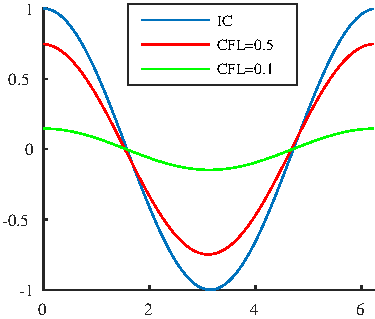
\includegraphics[scale=1]{fig/LAXF_IC2}
\caption{The solution of $u_t-u_x=0$ using the Lax-Friedrich scheme, coupled with the initial condition $\cos(x)+\frac{1}{4}\sin(mx)$, $m=\frac{N+1}{4}$ (left) and $m=\frac{N+1}{2}$ (right). In each figure, we plot the initial condition (blue $\color{blue} -$), and the solution using $CFL=0.5$ (red $\color{red} -$) and $CFL=0.1$ (green $\color{green} -$).}
\end{figure}

\begin{figure}
\centering
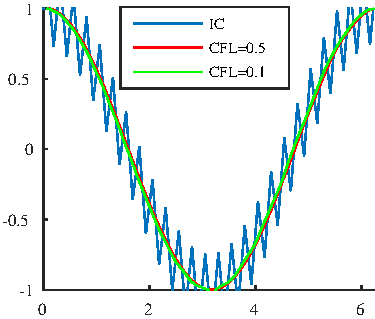
\includegraphics[scale=1]{fig/LAXW_IC1}
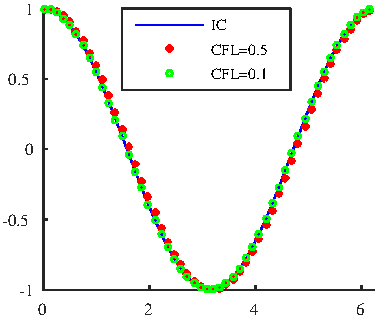
\includegraphics[scale=1]{fig/LAXW_IC2}
\caption{The solution of $u_t-u_x=0$ using the Lax-Wendroff scheme, coupled with the initial condition $\cos(x)+\frac{1}{4}\sin(mx)$, $m=\frac{N+1}{4}$ (left) and $m=\frac{N+1}{2}$ (right). In each figure, we plot the initial condition (blue $\color{blue} -$), and the solution using $CFL=0.5$ (red $\color{red} -$) and $CFL=0.1$ (green $\color{green} -$).}
\end{figure}

\end{enumerate}	
\end{enumerate}
	
	
	
	
\end{document}	
